\chapter{Data Analysis and the Results}
\label{chapter:Analysis}

In the section \ref{usecases}, we have listed the energy efficiency use cases. In chapter \ref{chapter:background}, we have explained the relevance of these use case to energy efficiency and also introduced and explained the basic concepts of suitable statistical and advanced analytics techniques to extract insights from data for these use cases. In chapter \ref{chapter:platform}, we have explained the implementation of a model Big Data platform for providing an environment to perform these analysis. In this chapter, we explain how we have performed our data analysis using the knowledge and capabilities developed through our work, which is explained in the previous chapters. We also present our results and their prospective applications. Before we go into the details of the use cases, analysis and the results, it is important that we explain the data sets.

\section{Data sets} \label{datasets}
In our analysis, we have used two distinct data sets provided by VTT. Both the data sets were collected by specialized devices installed on the test sites as part of the Green Campus initiative. The description of data sets are as follows.

\subsection{Data set 1: Hourly energy consumption data}
This data set contains hourly readings of the energy consumption taken by specialized meters installed by VTT (Technical Research Centre of Finland) on 40 different test sites in the cities of Espoo and Helsinki. Each site has at least one meter installed. Each installed meter on a particular site can record consumption of a specific energy type on an hourly basis. In some cases, a test site may have more than one meter even for same energy type. There are four energy types considered for test sites i.e. Electricity, Heating, Water and Reactive power. We consider only electricity and heating in the scope of this thesis. The heating usage is explained in terms of the electricity consumed to produce heating.  In the rest of this chapter, energy types will be termed as ``features'' and each record representing hourly consumption of a feature will be called an ``observation''.
There are approximately 1.2 million observations taken from the 144 installed meters on 40 different sites, during the 11 months period between 1st January 2013 till 30th November 2013.  Each row in the data represents an observation with the following information in exact sequence separated by commas: 

"Device ID","Destination Address","Building Name", "Meter", "type", "date", "hour", "Consumption"

A ``Device ID'' is the unique id for each installed device. To avoid confusion, the sites are being termed as buildings in the rest of the document, For sake of anonymity both ``Destination Address'' and the ``Building Name'' fields are masked as BuildingXX (where XX ranges from  01 to 40). ``Meter'' shows the nth number of the meter inside the same building. The field ``type'' labels the feature, while ``date'' refers to the calendar day in the format of YYYYMMDD, ``hour'' is the hour number of the day (0 to 23) and the ``Consumption'' is the consumption of the feature in respective units. Only electricity and electricity consumed for heating is considered in this paper so units are 10xWh (Watt hour).
To fix the scale of consumption to Kilo Watt Hour, each consumption value should be divided by 100. 

The data set is not consistent and has an unequal number of the observations for some buildings per energy type per day. Figure~\ref{fig:incon} illustrates the summary of this data set and shows the inconsistencies. From the figure ~\ref{fig:incon}, we can see that the number of the records for each building are not equal. In an ideal data set they should be the same. The inconsistencies occur because of the multiple number of devices collecting data, however exploratory analysis reveals that for some of the buildings, the consumption values were totally missing. In some other cases, all the days in the 11 months period were not available. Similarly all hours in a day were not fully captured for some buildings.

\begin{figure}[!ht]
    \begin{center}
      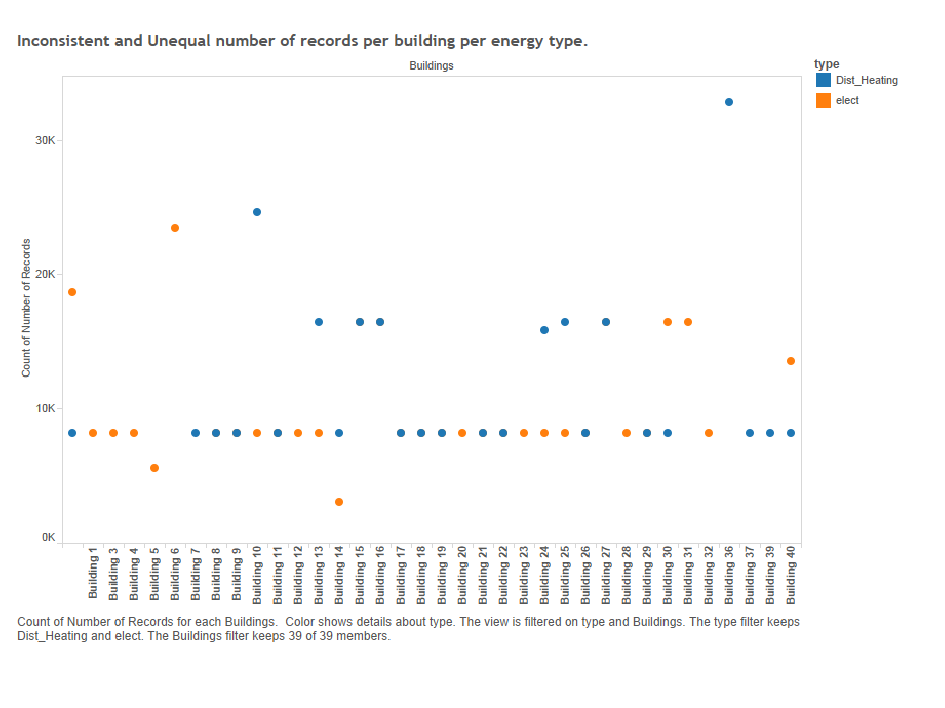
\includegraphics[width=\textwidth]{images/incon.pdf}
      \caption{Data Inconsistencies in hourly energy consumption data.}
      \label{fig:incon}
    \end{center}
  \end{figure} 
Apart from the inconsistencies shown by number of the records, some building names and addresses were also missing. To handle inconsistent data, we had to adapt our analysis using aggregation techniques like averaging. We shall also explain other data cleaning and pre-processing techniques in section \ref{cleaning}. The implementation level details of data are available in Appendix \ref{chapter:appendixc}

To support this data set for the analysis, we have also collected the real estate data that includes floor area of each building included in this data set. The Real Estate data was collected using the following Espoo city information website.
\url{http://https://arska.espoo.fi/}


\subsection{Data set 2: Device level data} \label{nialmset}
This data set contains device level consumption of the electricity collected from a residential apartment included as a test site for the VTT's Green Campus initiative. Device level means that the electricity consumption was collected for various home appliances used in that apartment. These appliances were differentiated on the basis of their respective electrical signal thumbprint using NIALM metering devices described in section \ref{greencamp}. The data was collected from 1st May 2013 to 30th April 2014 in form of a text file from the VTT's data webservice. The different fields in the data were separated by ``;''. The data set has the following fields.

``Devic'';``Timestamp'';``Consumption(Wh)''

The ``Device'' field is a label for the respective home appliance e.g. refrigerator, freezer, TV, and stove etc. ``Timestamp'' contains the date, hour, minutes and seconds of the recorded data in the  YYYY-MM-DD HH:MM:SS format. The ``Consumption\((Wh)\)'' field contains the value of electricity consumed and recorded at that instance of time. The devices that are used on demand for example a TV, stove, coffee maker etc. records the consumption values right after the end of the respective usage session. For continuously used devices like refrigerators and freezers etc. NIALM devices have their inbuilt mechanism to keep recording the data. For our research we take the data record as it appears in the data set.   

\section{Use Case Categories}

As listed previously in the section \ref{usecases}, the following are the main use cases for our research.

\textbf{Use Case 1:} Understanding the seasonal energy usage patterns and their sensitivity with outside temperature.

\textbf{Use Case 2:} Understanding the characteristics of the buildings using daily energy consumption pattern.

\textbf{Use Case 3:} Calculating the base load of the buildings to identify off-peak hours usage when users are not in the building.

\textbf{Use Case 4:} Classifying the buildings on the basis of energy efficiency and analyse seasonal shifts in this classification.

\textbf{Use Case 5:} Forecasting the daily energy consumption of various household appliances on the basis of the previous consumption patterns.

Data set 1 was used for the use cases 1,2,3 and 4, while data set 2 was used only for the use case 5. In a similar way we grouped the use cases into two categories for analysis. Use cases 1 to 4 were referred to as ``Energy Consumption patterns and classification of the buildings on the basis of energy efficiency''. While use case 4 was labelled as ``Prediction model for forecasting  the energy consumption of the household devices ''


\section{Energy Consumption patterns and classification of the buildings on the basis of energy efficiency}
In the section \ref{ecoeff}, we have discussed the concept of energy efficiency in context of the ecological factors. In the section \ref{seasonal}, we have discussed the impact of outside temperature on energy usage. Similarly we have established the relationship between daily load, base load and energy efficiency in the section \ref{daily}. Now using all these concepts together, we try to analyse data set 1 and detect the daily and seasonal trends for energy usage. We also try to find out the base loads for the buildings to see which building is consuming more energy during the off peak hours when users are not present in the building. Finally we attempt to classify the building on the basis of energy efficiency as per section \ref{classify}. The following subsections will describe the each step along with explanation of the analysis and results.
\subsection{Data cleaning and pre-processing} \label{cleaning}
For preparing a tidy data set for the analysis, the following steps were performed:
\begin{enumerate}
\item We intended to perform the analysis for electricity and heating features, so the relevant observations were extracted from the data. In the rest of the document, we only consider these extracted observations.
\item To check the consistency and quality of the data, a quick statistical analysis was performed. The result of the analysis is illustrated in figure~\ref{fig:incon}.
\item The consumption scale was set to KWh (Kilo Watt Hour).
\item For each feature, the distinct buildings were listed to see how many buildings have each type of feature available. The result shows that 32 out 40 building has observations available for electricity while 24 has observation for heating. The observations for those building were extracted which have records available for both the features. In some of the observations there were empty ``Destination Address'' and ``Building Name'' fields. Such observations were tagged as ``Unknown''. 
\item There were some other pre-processing steps that are explained with their respective use cases.
\end{enumerate}

\subsection{Seasonal variation in energy consumption}
Seasonal variation in the use of electricity is a very obvious phenomenon. However the important aspect for our analysis was to first see the sensitivity of energy usage with change in outside temperature as per use case 1 and then see the impact of the seasonality on the classification of building on the basis of energy efficiency i.e. to check if a building of a particular class shifts to another class with change in the external temperature. This provides the basis for use case 4. Since all of the test buildings are in cities of Helsinki and Espoo which are geologically located close to each other, so it can be safely assumed that both city has similar temperatures throughout the year. The upper graph in figure~\ref{fig:season} shows the aggregated consumption for all the buildings. Two separate lines represent electricity and electricity used for heating respectively. While the lower graph shows the average temperature of Helsinki and Espoo during the same time of the year. The temperature data was collected using the Finnish Meteorological Institutes's (FMI) data API.       
 
\begin{figure}[!ht]
    \begin{center}
      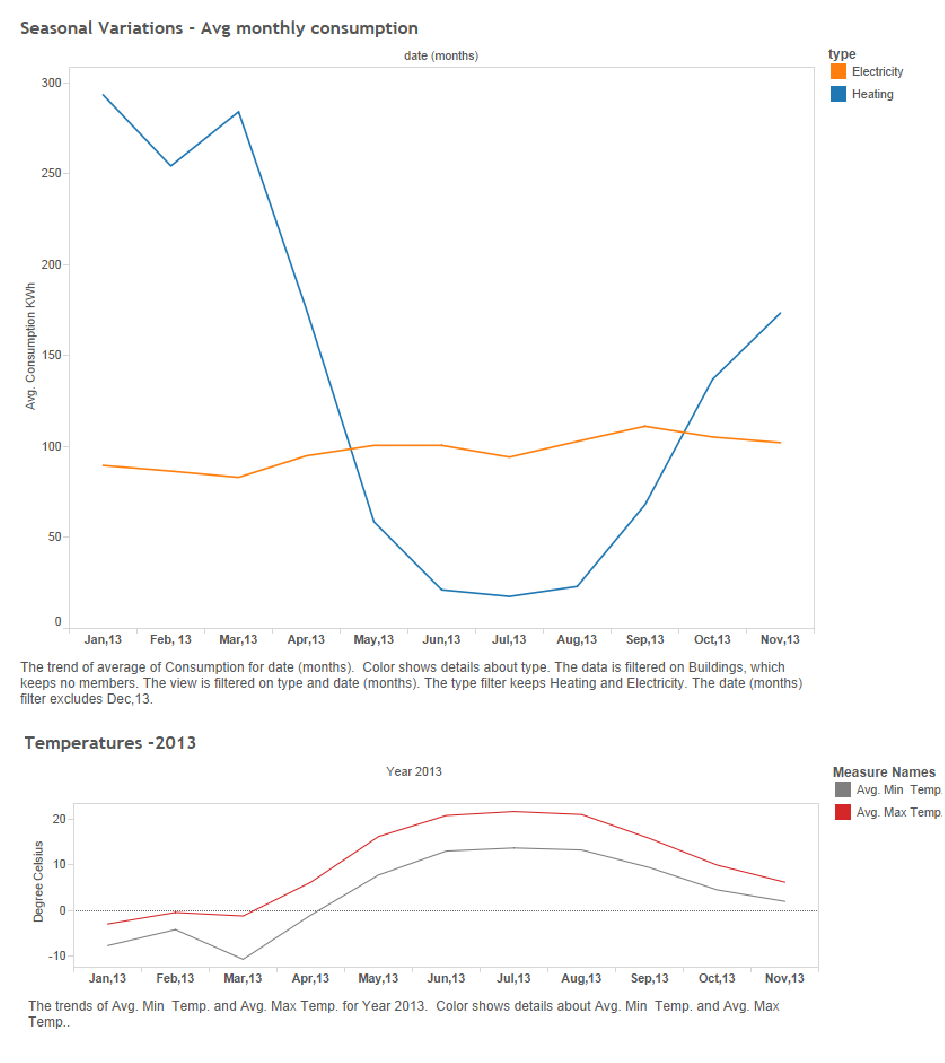
\includegraphics[scale = 0.7]{images/season.pdf}
      \caption{Seasonal patterns in usage of electricity and electricity used for heating.}
      \label{fig:season}
    \end{center}
  \end{figure} 

Figure ~\ref{fig:season} shows that electricity used for heating is more sensitive to temperatures than electricity  used for the other purposes. The general purpose electricity consumption shows a relatively stable trend through out the 11 months period. For the service providers, improving heating distribution and usage systems can contribute more to energy efficiency. 

\subsection{Daily trends}
Detecting and projecting the daily trends from data set 1 can provide us two very important insights that corresponds to use cases 2 and 3. It can help to suggest the characteristics of a building without having any prior information of the building. For example if the use of energy is higher during the work hours of the working days and lesser during night times and on the weekends, then we can suggest that the building is an office building. Secondly, the base load analysis can refer us to building where there could be possible electricity leakages. Rectifying such issues can improve the overall energy efficiency of the buildings.

In our analysis we detected the daily trends of the buildings by averaging the consumption of each building separately for each hour of the day. Normalizing the data for missing values was very important, so instead of averaging with the total number of days for each building, we took averages for the number of days for which data is available. 

\begin{figure}
        \centering
        \begin{subfigure}[b]{0.45\textwidth}
                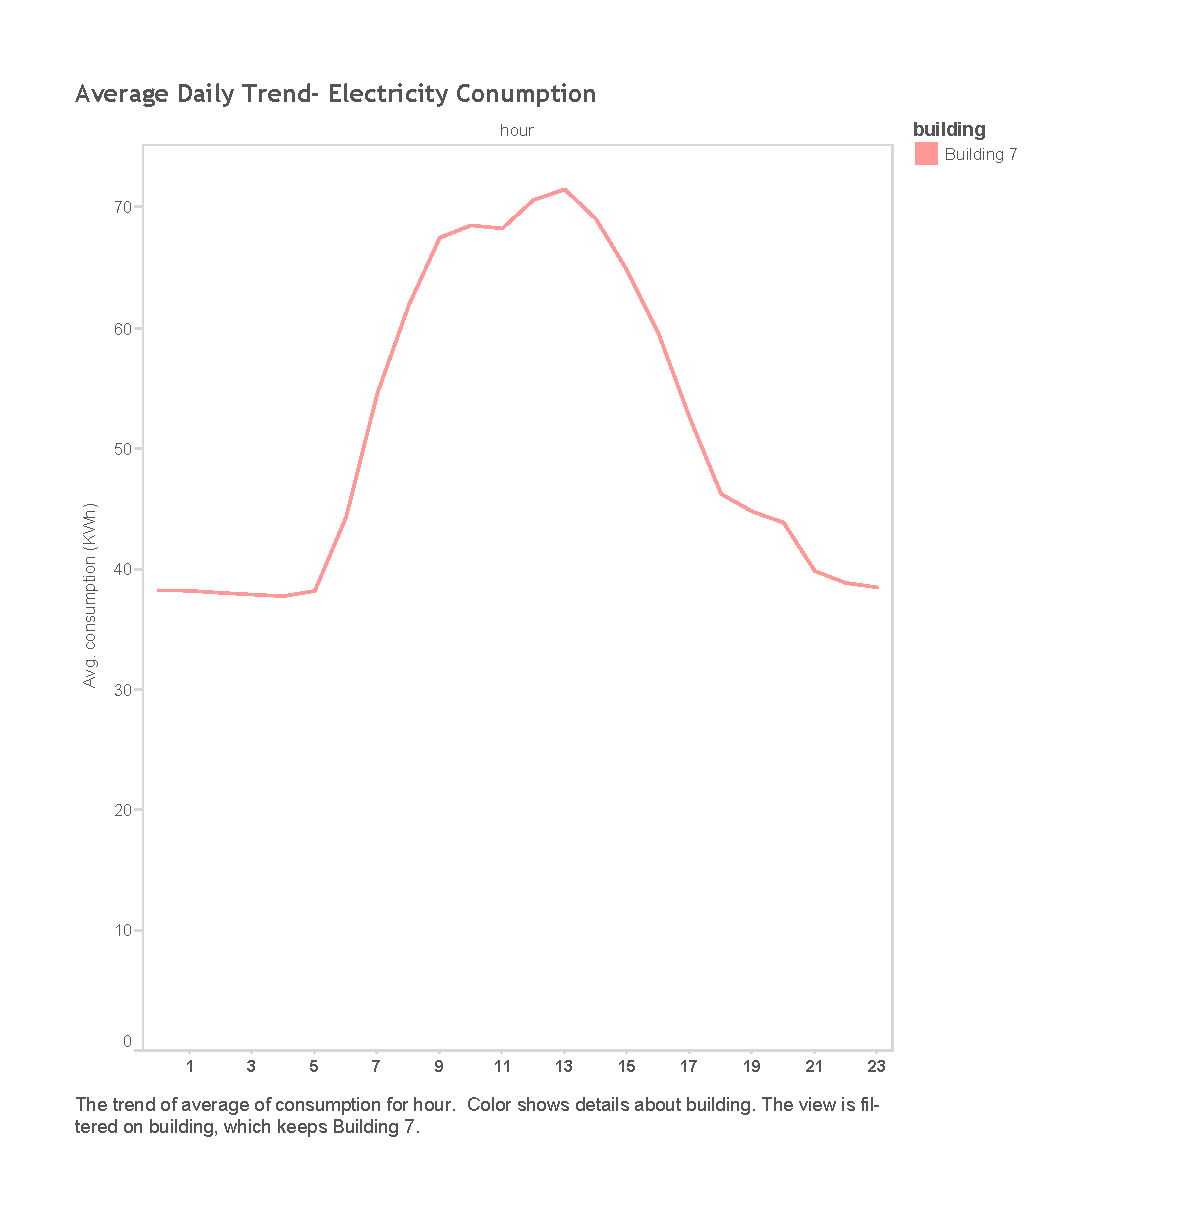
\includegraphics[width=\textwidth]{images/db6_elec.pdf}
                \caption{Building 6: Daily electricity consumption trend}
                \label{fig:elec6}
        \end{subfigure}%
        \begin{subfigure}[b]{0.45\textwidth}
                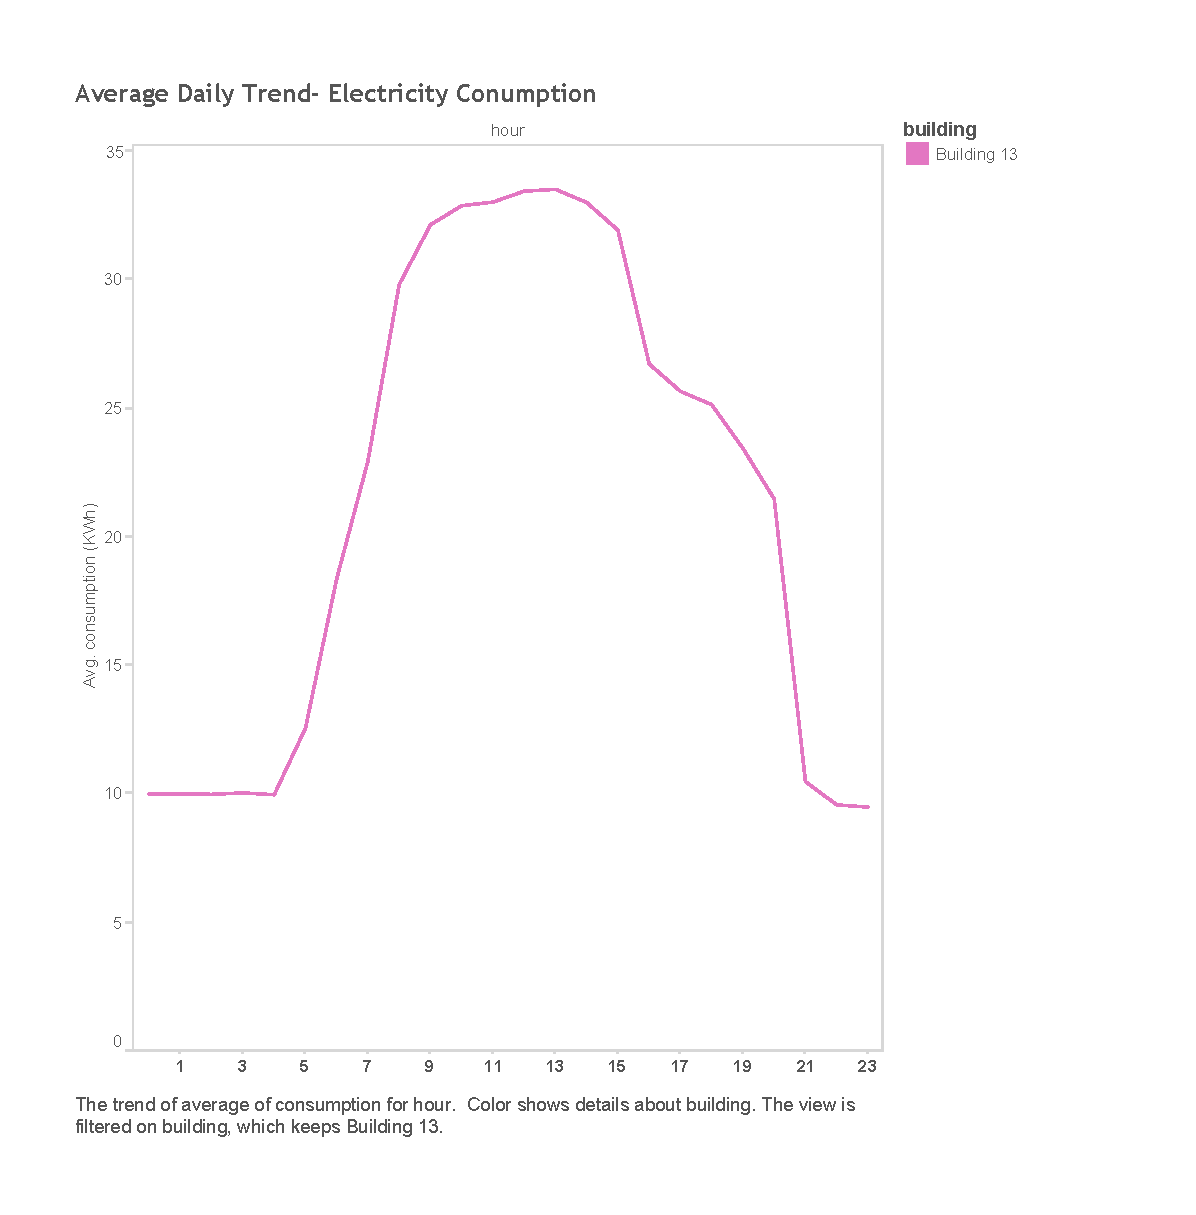
\includegraphics[width=\textwidth]{images/db13_elec.pdf}
                \caption{Building 13: Daily electricity consumption trend}
                \label{fig:elec13}
        \end{subfigure}
        
        \begin{subfigure}[b]{0.45\textwidth}
                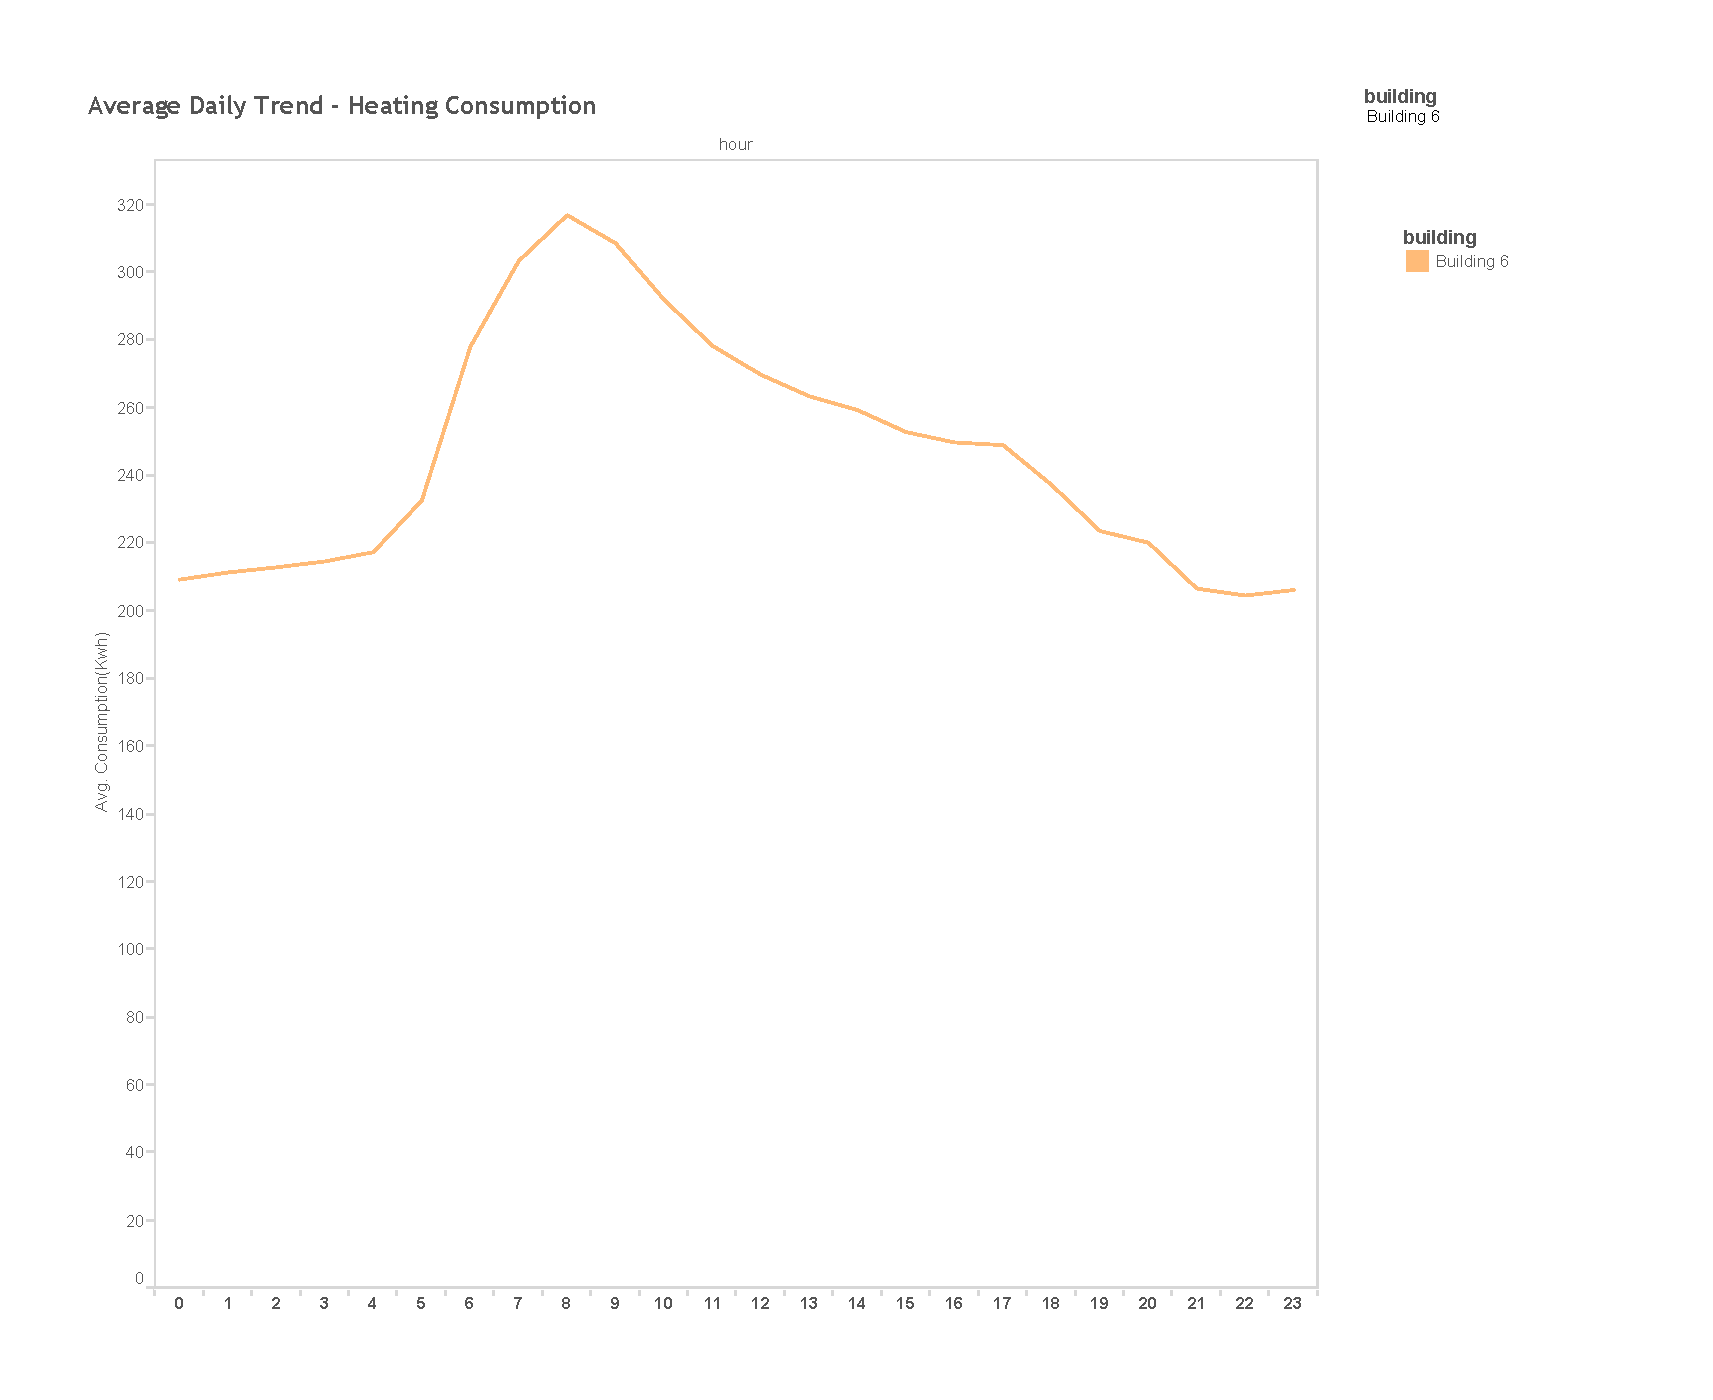
\includegraphics[width=\textwidth]{images/db6_heat}
                \caption{Building 6: Daily electricity for heating consumption trend}
                \label{fig:heat6}
        \end{subfigure}
        \begin{subfigure}[b]{0.45\textwidth}
                        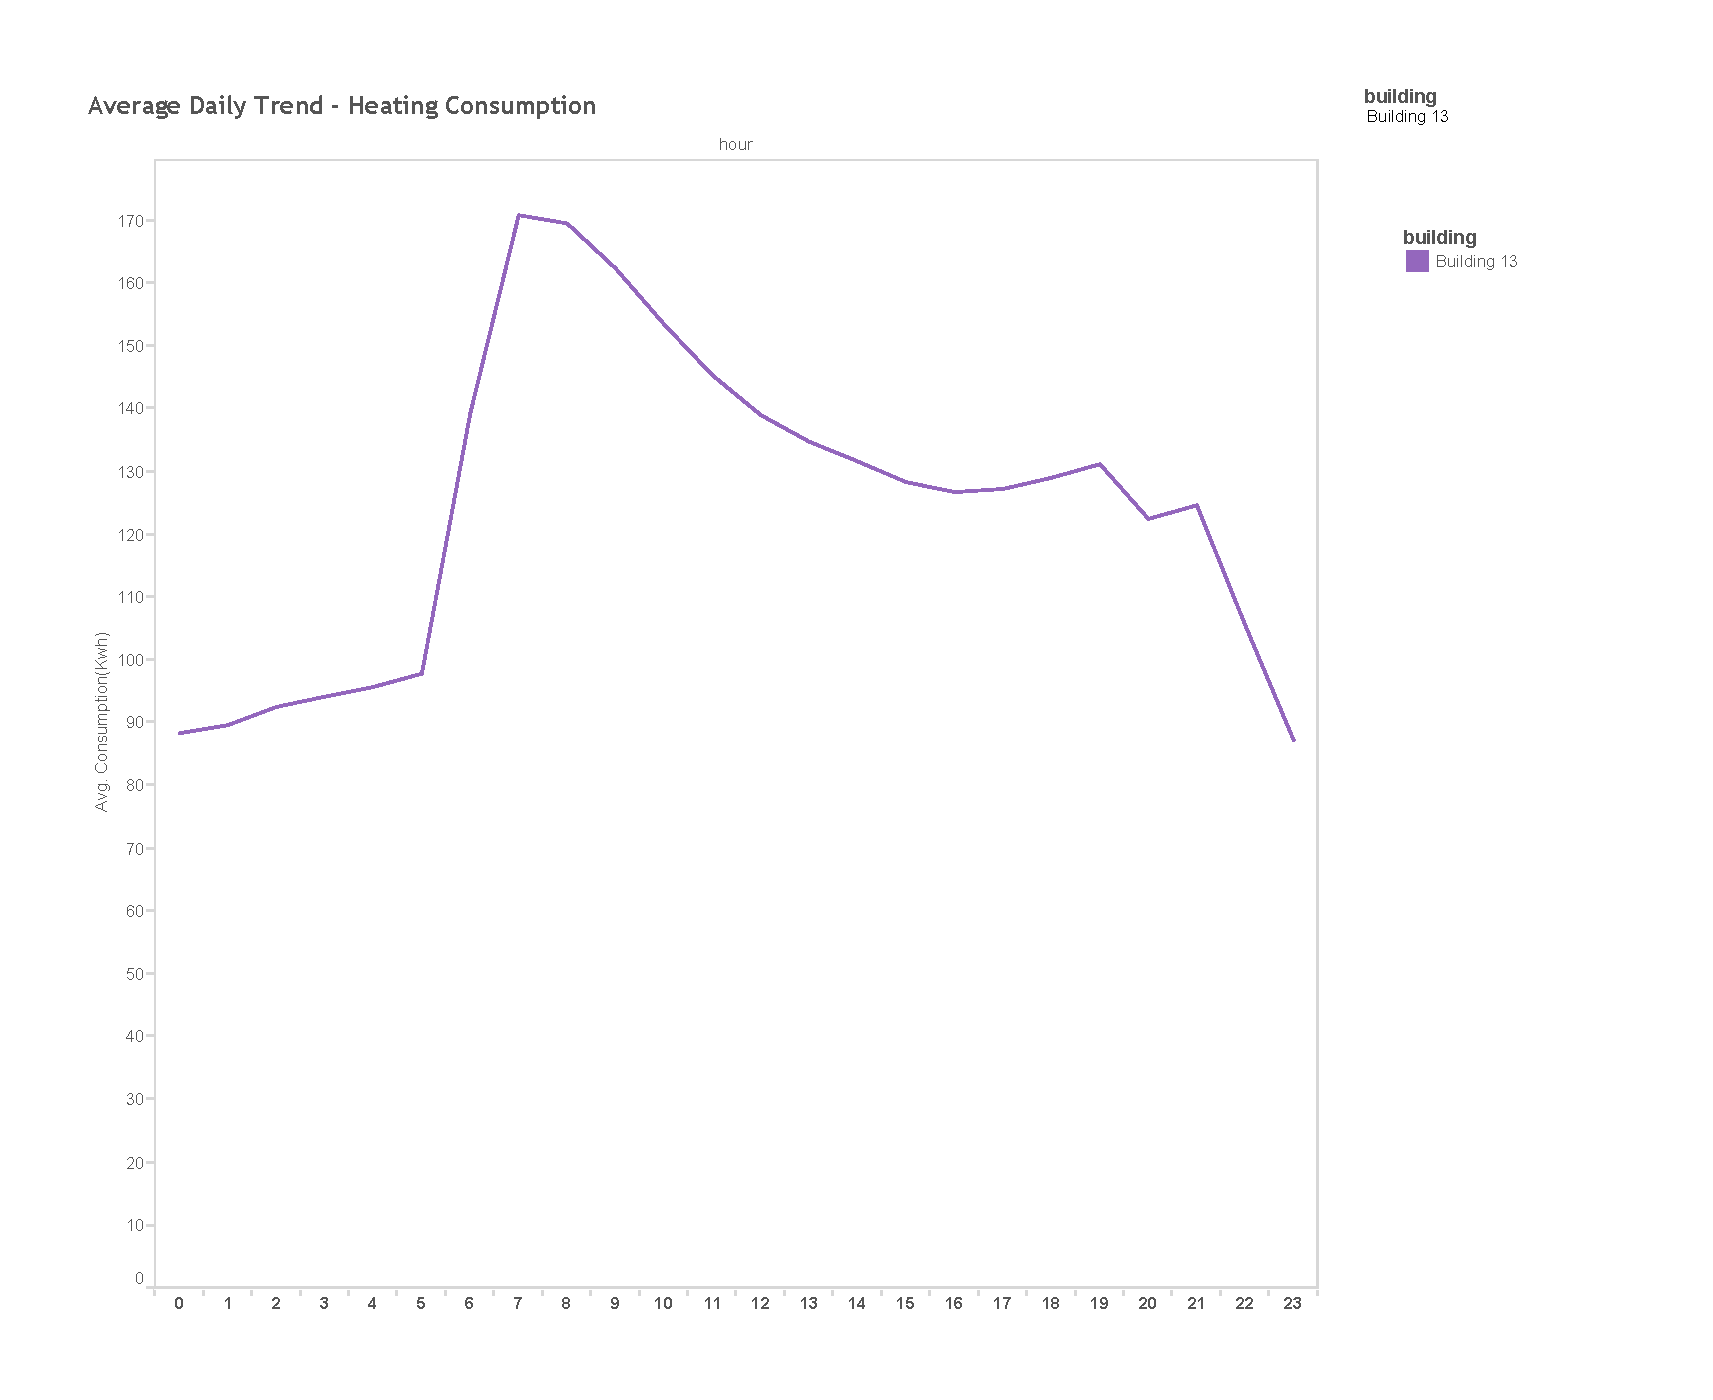
\includegraphics[width=\textwidth]{images/db13_heat}
                        \caption{Building 6: Daily electricity for heating consumption trend}
                        \label{fig:heat13}
       \end{subfigure}
     \caption{Daily energy consumption patterns}\label{fig:animals}
\end{figure}

Figures \ref{fig:elec6} and \ref{fig:elec13} show the average daily electricity consumption of the two buildings from our data i.e. Building 6 and 13 respectively. While  figures \ref{fig:heat6} and \ref{fig:heat13} show the electricity consumption for the heating of the same buildings. Both type of consumption are higher during office hours suggesting the purpose of building.  While each building has different base loads. Base load hours are very visible in the daily trends graphs. An interactive dashboard to observe the trends for all the buildings is available on the following website:

\url{http://https://arska.espoo.fi/}

A quick exploratory analysis of the trends suggests that all buildings are office buildings. Secondly the daily base load hours are hour 0, 1, 2, and 23. The base loads can then be calculated by averaging the consumption for these hours. Appendix \ref{chapter:appendixd} contains the list of calculated base loads for each of the buildings in each month of the year within available data.

\subsection{Classification of buildings on basis of energy efficiency}
Classification on the basis of energy efficiency can be used as a tool to benchmark and segregate the inefficient energy consumption units from the efficiently performing buildings. Such classification can narrow down the scope of research for finding the possible energy leakages and faults. We discussed the main concepts and the K-means clustering technique, we used for our analysis in section \ref{classify}. The existence of some similarity is a pre-condition for any cluster analysis technique. To test this on our data set we calculated the average hourly energy efficiency using equation ~\ref{spec_energy} for each building. Figure~\ref{fig:hr_m2} confirms the availability of similarly behaving buildings in terms of energy efficiency. 
\begin{figure}[!ht]
    \begin{center}
      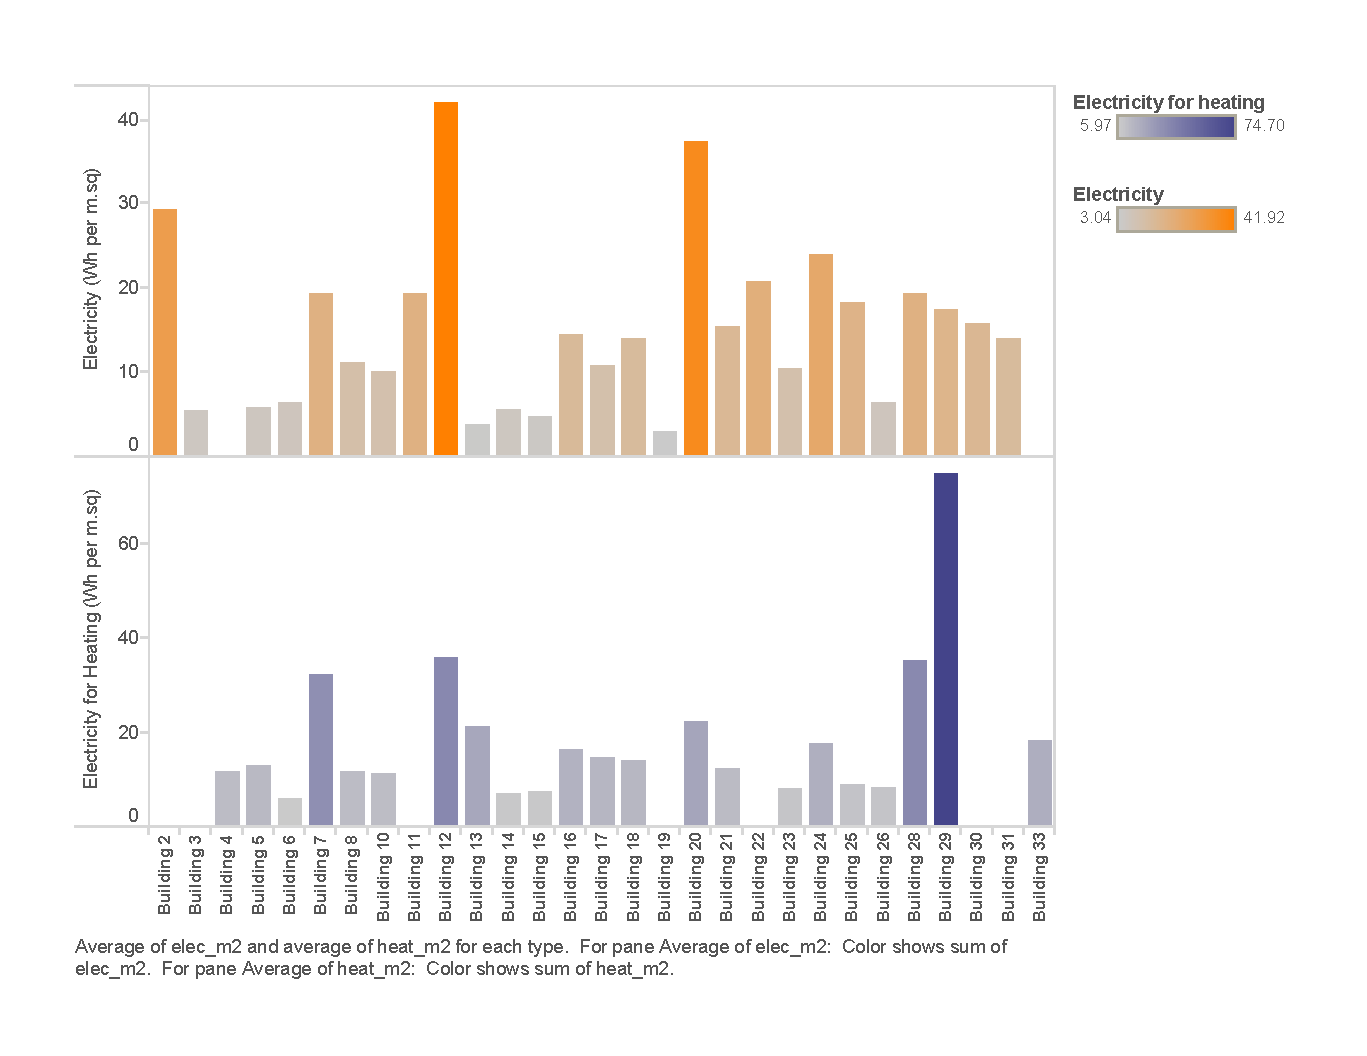
\includegraphics[scale = 0.6]{images/hr_m2.pdf}
      \caption{Energy efficiency of buildings with hourly average consumption.}
      \label{fig:hr_m2}
    \end{center}
\end{figure} 

\subsection{Data processing for cluster analysis}
The K-means algorithm needs input data in the form of a matrix, where the values of each feature are defined in their respective columns, while each row represents a data point that will be grouped together in the form of clusters. In our case we have two energy features i.e. electricity and the electricity used for heating. While the average monthly energy efficiency value for each month and each building is represented by a row in the input matrix. The reason for considering the average monthly values for buildings is to analyse the energy efficiency of the building throughout the 11 months period. So in this way our input matrix consisted of: 
\begin{lstlisting}
Number of rows, i = Number of buildings x 11 
Number of coulmn, j = 2
\end{lstlisting}
Following are the main data processing steps for our cluster analysis. These steps were performed on the data set that we have as output of the preliminary data pre-processing described in section \ref{cleaning}.
\begin{enumerate}
\item We segregated the electricity and electricity used for heating records from each other.
\item We calculated the average daily consumption for each building and each energy type first. Then calculated the average monthly consumption in similar way. It is important to normalize the data by taking the averages on the basis of number of records available for the hours within a day and then the days within a month. 
\item We then arranged calculated average monthly consumption values for each energy type in form of a matrix labelled with building names and month names as the separate columns. We called this matrix as the ``Energy Consumption Matrix''.   
\item At this stage our Energy Consumption Matrix had few buildings for which consumption values were missing for either type of energy feature. We removed these building to avoid inconsistency in data for the cluster analysis. 
\item We then introduced the real estate data i.e. ground floor area of the respective buildings into our energy consumption matrix. Using equation ~\ref{spec_energy}, we calculated the energy efficiency values for each energy feature. We termed the resulting matrix as the ``Energy Efficiency Matrix''.
\item Until this point, we had energy efficiency in units of Kilo Watt hour per square metre. We then converted the values into Watt hour per square metre. This was an optional step and it was performed just to avoid handling small decimal values.
\item To prepare the final input matrix we removed the labels and left two columns of energy efficiency values for the two target energy features.
\item To finalize the K-means input matrix, we used the R programming \textbf{scale()} function to set the unit variance for all the matrix elements. This function could have also normalized the scale of the measurements, however in our case it was already a similar unit for both energy types i.e. \((Wh/m^2)\).        
\end{enumerate}
\subsection{K-means clustering analysis and results}
Our use case requirement was to classify the buildings into four categories of high efficiency, moderate efficiency, low efficiency and poor efficiency buildings. So we had the pre-defined K value of 4. We applied K-means clustering on our input matrix using R programming \textbf{kmeans()} function.

As a post processing step we combined the resulting cluster values to the energy efficiency matrix in front of their respective labels (Building Name + Month Name) and energy efficiency values (electricity and electricity used for heating). We termed this matrix as the ``Clustered Matrix'. The Clustered Matrix was then fed into Tableau public as a CSV file to create an interactive dashboard and visualisations. Figure~\ref{fig:kmeans} visualises the result of clustering.  

\begin{figure}[!ht]
    \begin{center}
      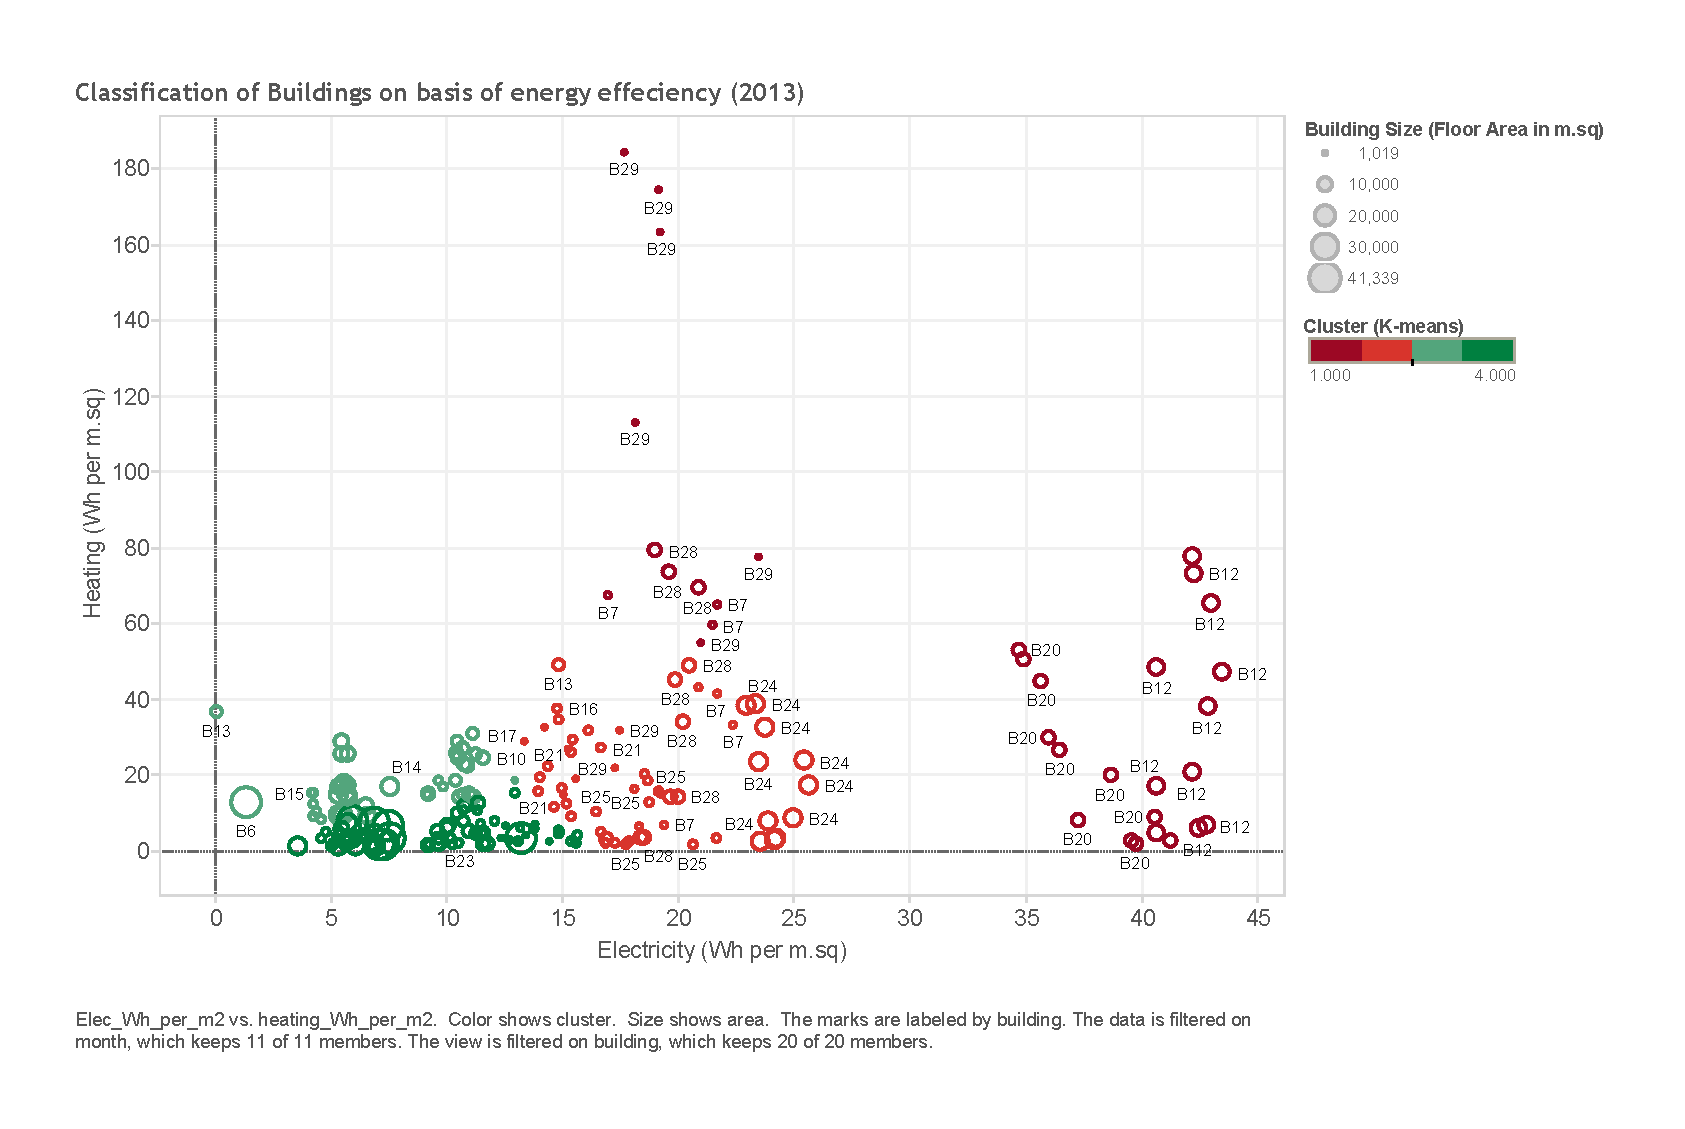
\includegraphics[width=\textwidth]{images/kmeans.pdf}
      \caption{K-means clustering, Average monthly energy efficiency per each building.}
      \label{fig:kmeans}
    \end{center}
\end{figure} 

Each bubble on the graph  in Figure \ref{fig:kmeans} represents a month's average energy efficiency value for a particular building. The colour of the bubble represent the respective cluster or class. While size of the bubble represents the size of the building. The cluster numbers range from 1 to 4, where 4 represents the highly efficient class and 1 is for the most energy inefficient class of the buildings. Figure ~\ref{fig:kmeans_jan} shows the one month subset of the clustered values. Each buble represent average energy efficiency in the month of January. 
\begin{figure}[!ht]
    \begin{center}
      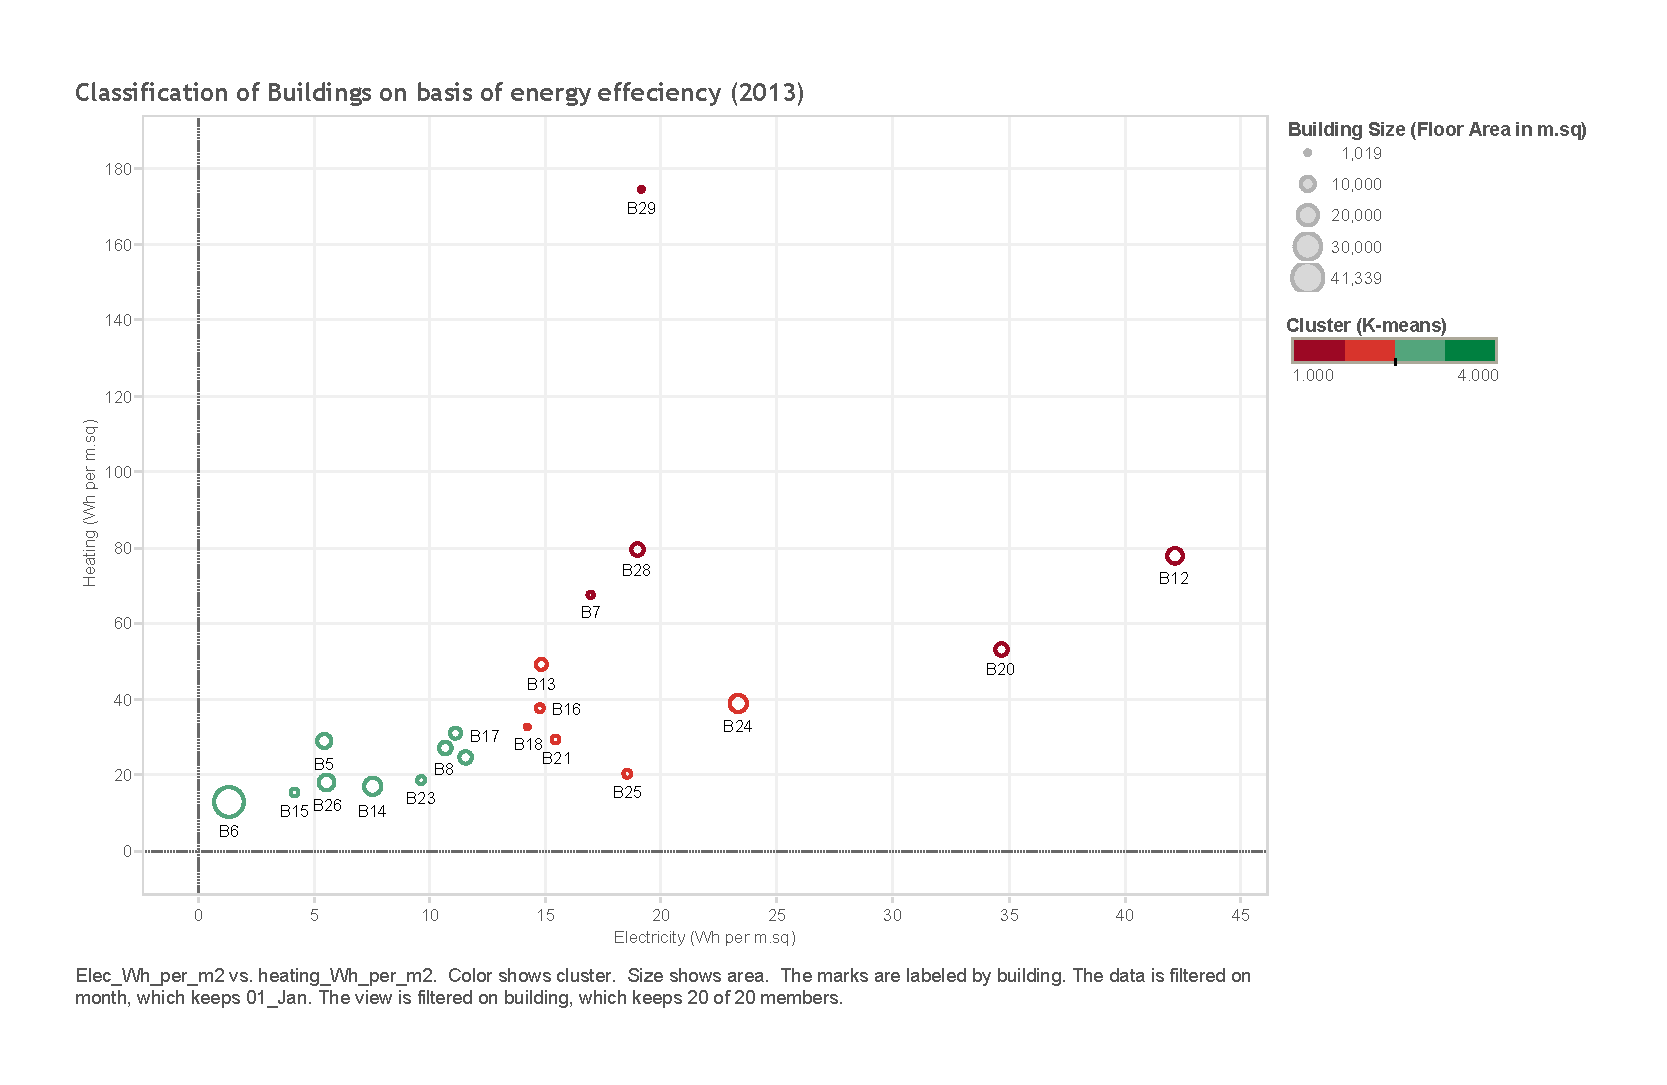
\includegraphics[width=\textwidth]{images/kmeans_jan.pdf}
      \caption{K-means clustering, A one month view.}
      \label{fig:kmeans_jan}
    \end{center}
\end{figure} 

\textbf{Insight:} Figures~\ref{fig:kmeans} and ~\ref{fig:kmeans_jan} reflect a very important insight; that some of the bigger size buildings are in high or moderate efficiency clusters while some of the smaller buildings are in inefficient clusters. Such extreme cases can be good targets for case studies. The low efficiency buildings may have some energy leakages, faults or inefficient usage practices while the high efficiency buildings may suggest good practices for using energy. 

As part of the use cases, we also studied the change behaviour of the buildings with the external temperatures, while using the same cluster analysis. Figure~\ref{fig:clustershift} illustrates the behaviour of different buildings during the 11 month period. Figures ~\ref{fig:tri_1} and \ref{fig:tri_2} present the behaviour of Building 29 and Building 7 respectively. Both the buildings shift among three different clusters. While figures \ref{fig:dbl} and \ref{fig:single} represent the buildings 16 and 24 that show shift between two clusters and no clusters  respectively.
\\
\textbf{Insight} Figure ~\ref{fig:clustershift} shows the fact that buildings are not equally energy efficient or inefficient throughout the year. 

\begin{figure}
        \centering
        \begin{subfigure}[b]{0.45\textwidth}
                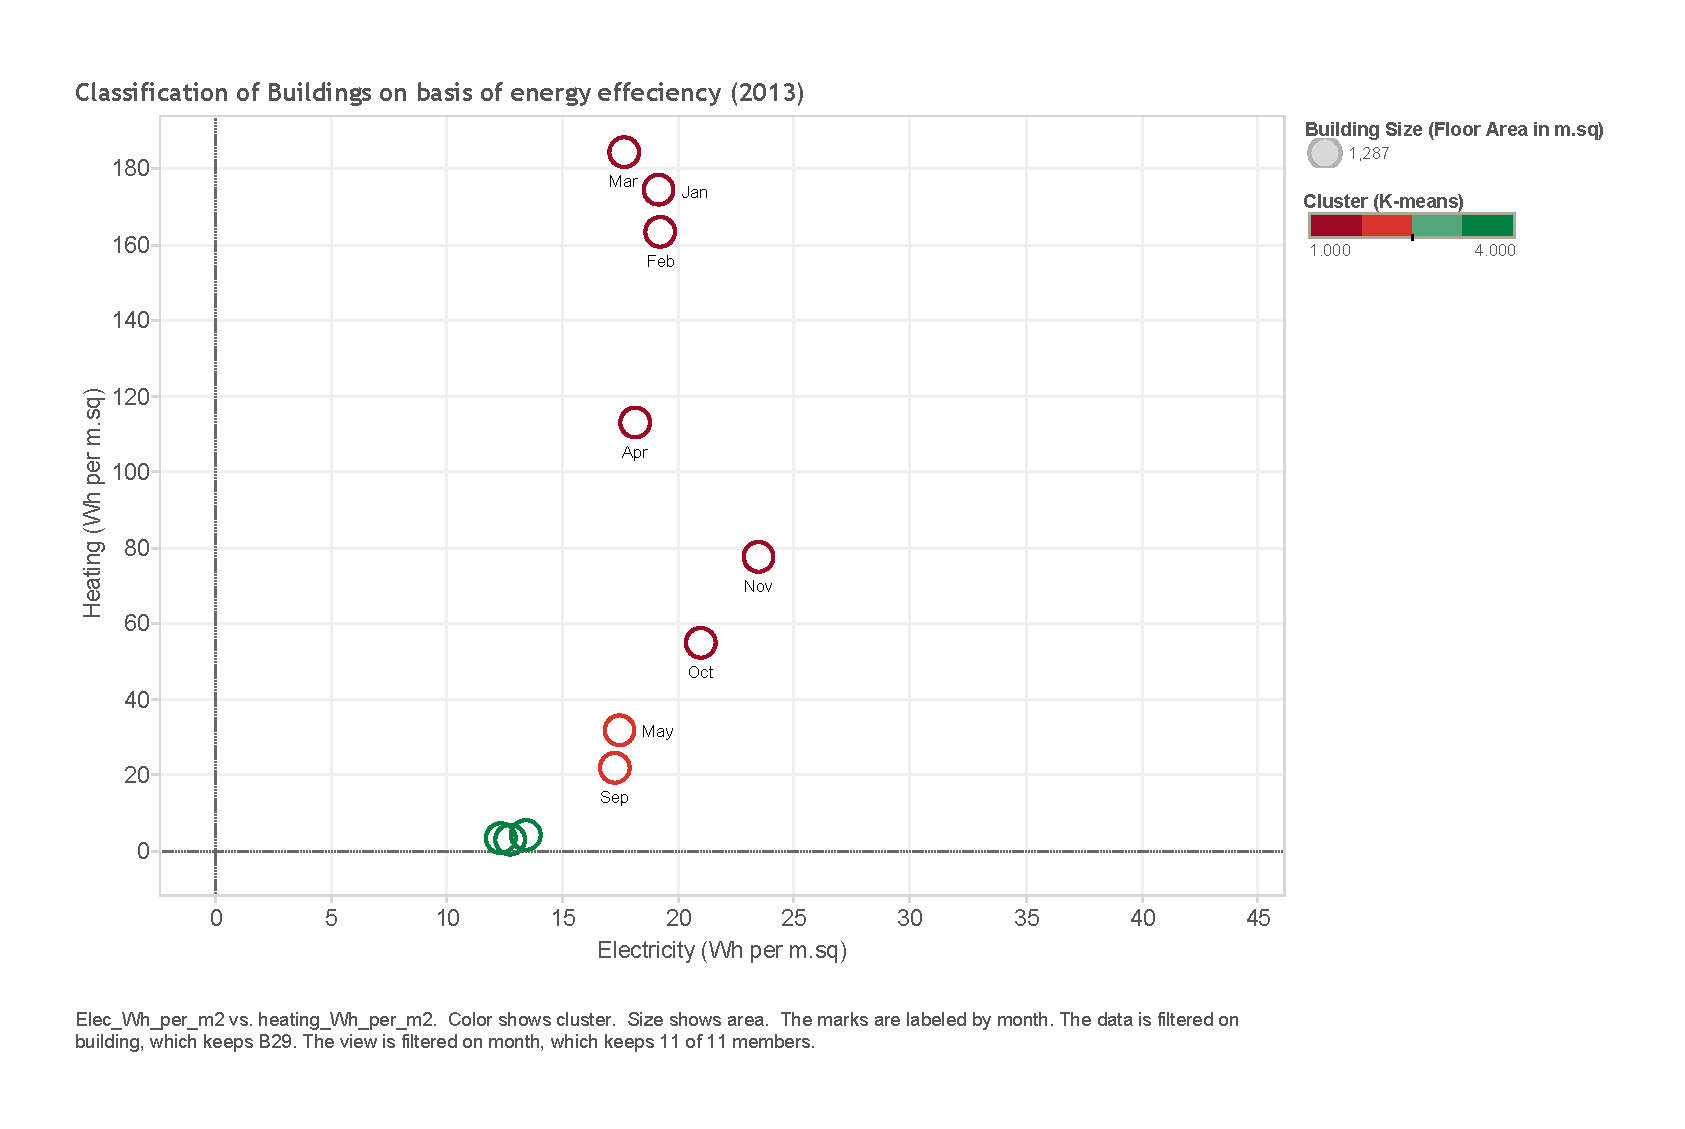
\includegraphics[width=\textwidth]{images/kmeans_b29_3c.pdf}
                \caption{Building 29:  Triple shift}
                \label{fig:tri_1}
        \end{subfigure}%
        \begin{subfigure}[b]{0.45\textwidth}
                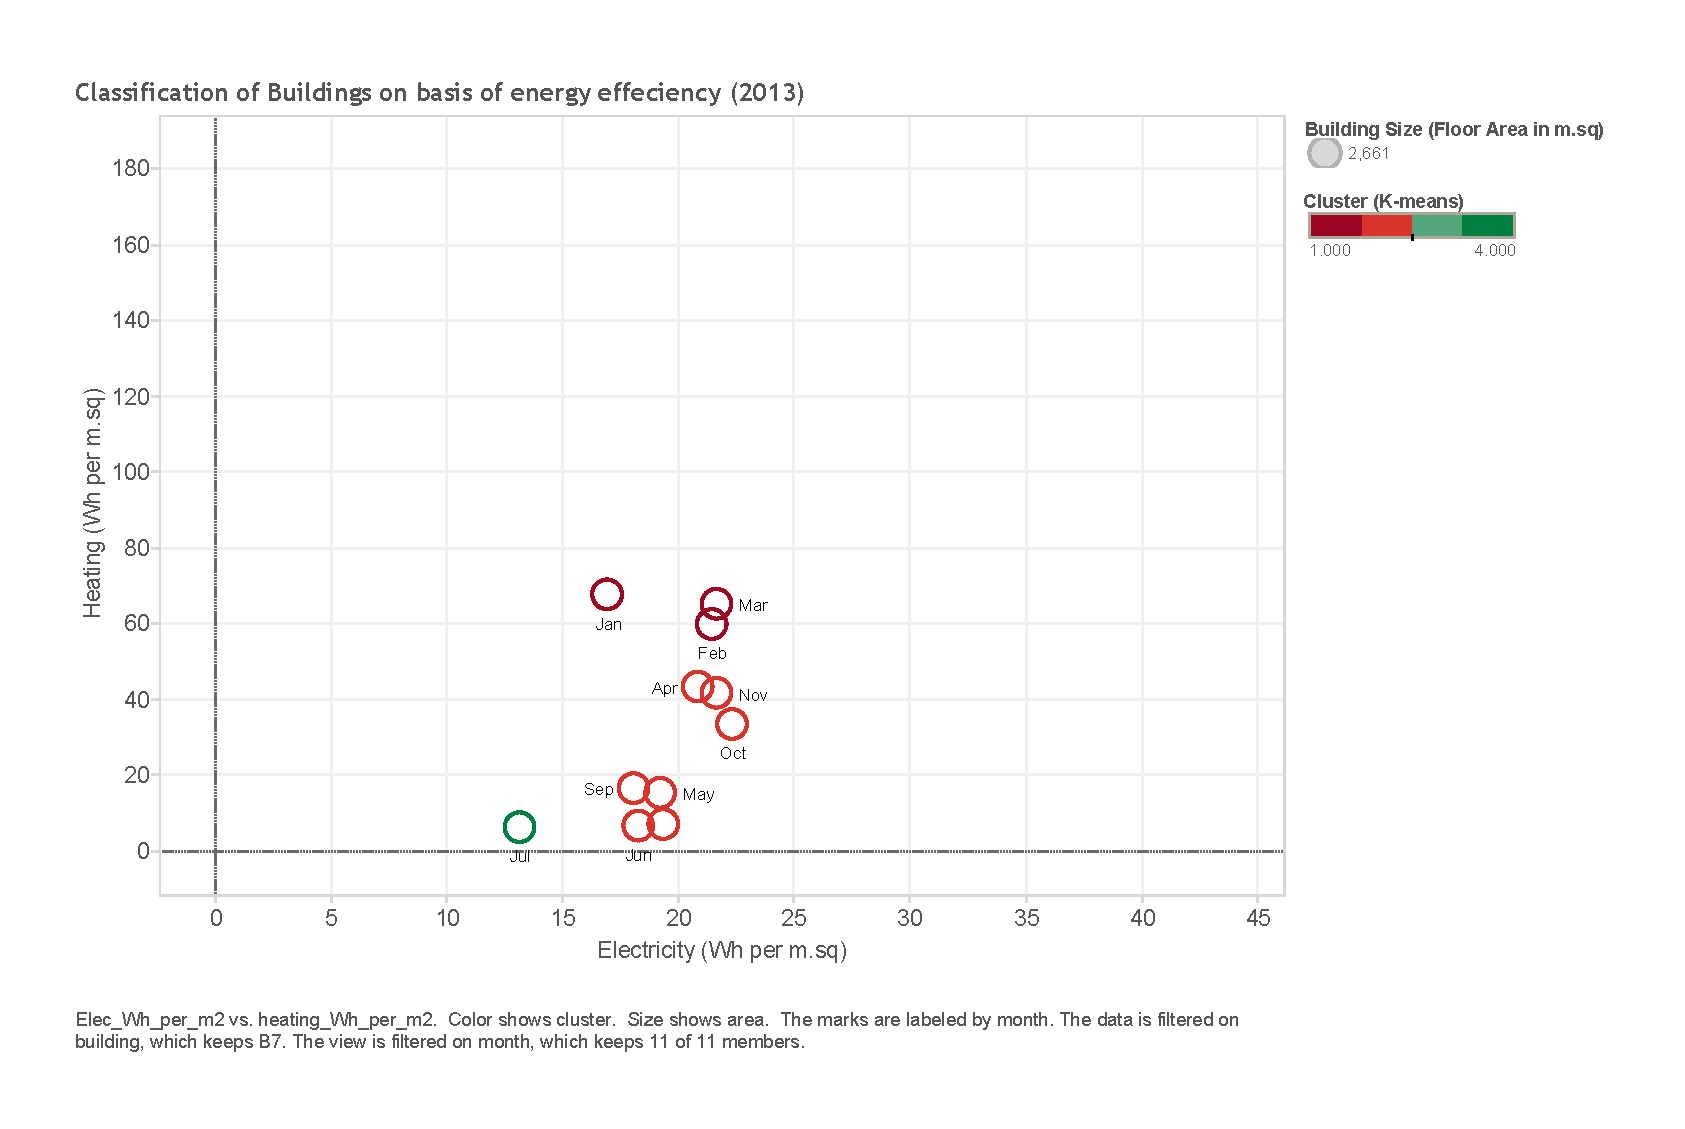
\includegraphics[width=\textwidth]{images/kmeans_b7.pdf}
                \caption{Building 7: Triple shift}
                \label{fig:tri_2}
        \end{subfigure}
        
        \begin{subfigure}[b]{0.45\textwidth}
                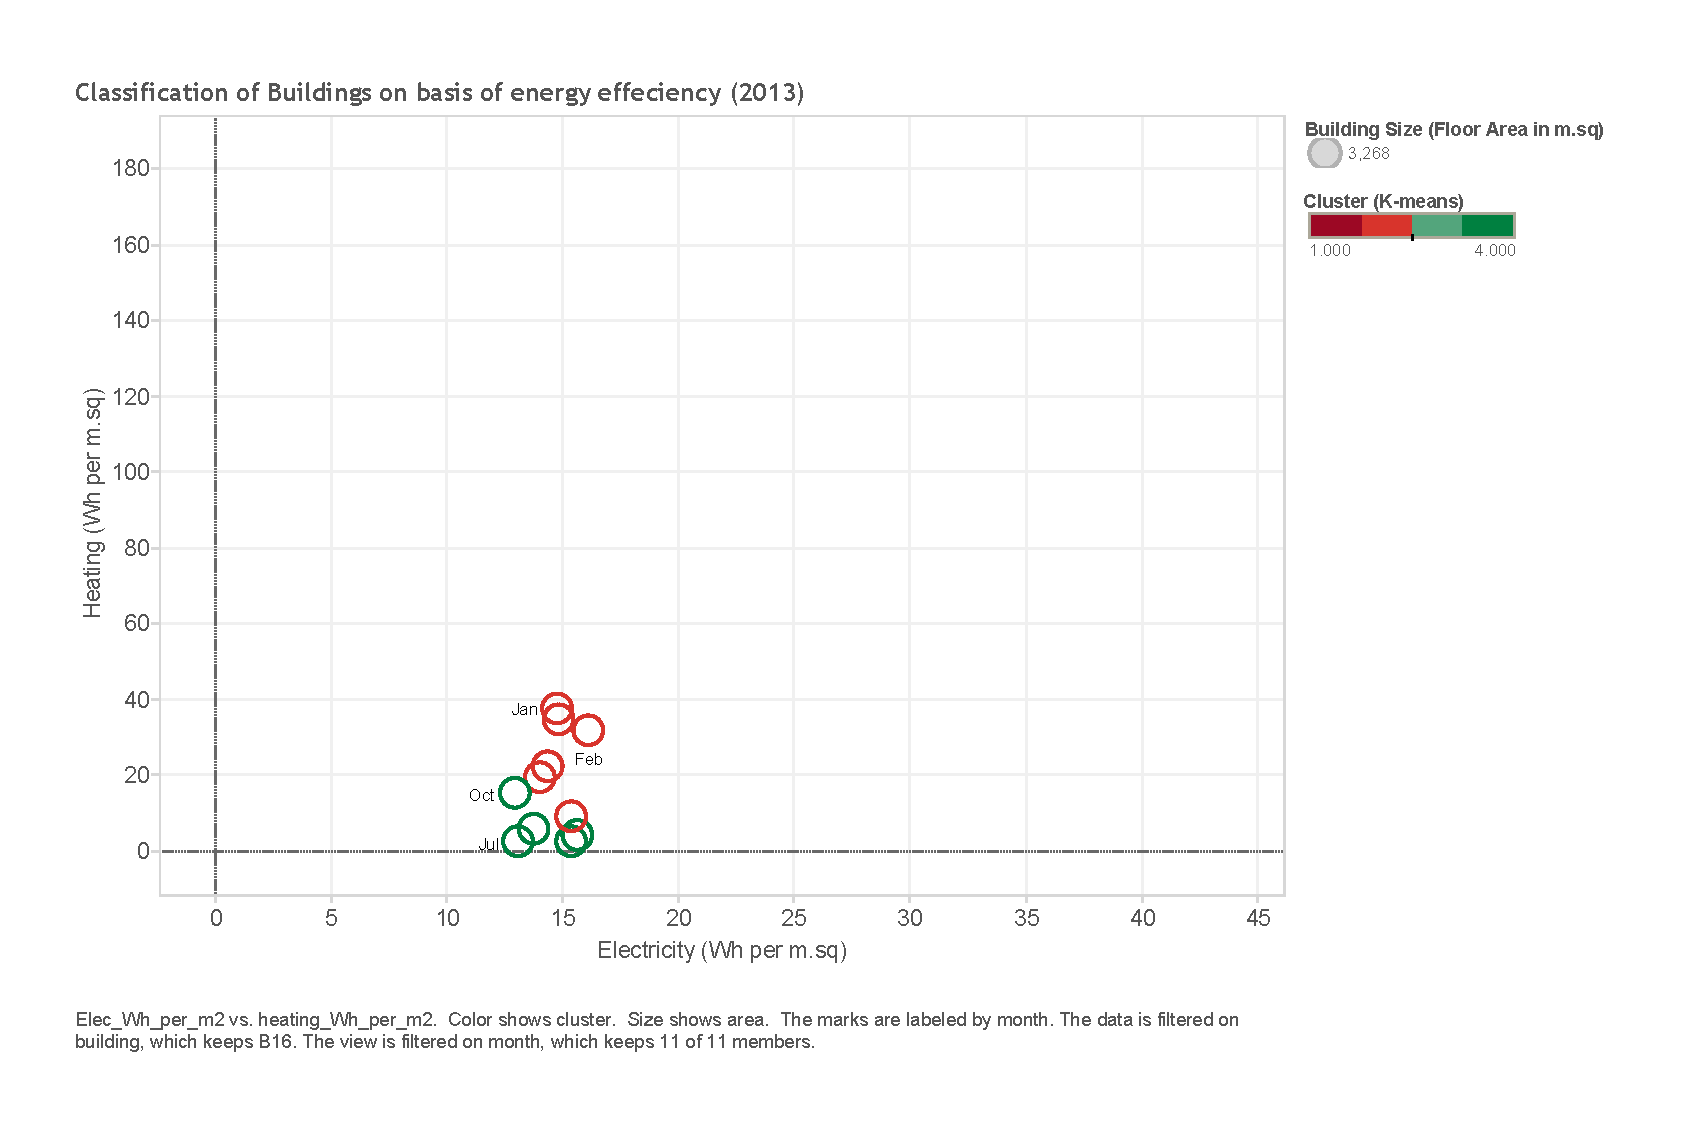
\includegraphics[width=\textwidth]{images/kmeans_B16_2c.pdf}
                \caption{Building 16: Double shift}
                \label{fig:dbl}
        \end{subfigure}
        \begin{subfigure}[b]{0.45\textwidth}
                        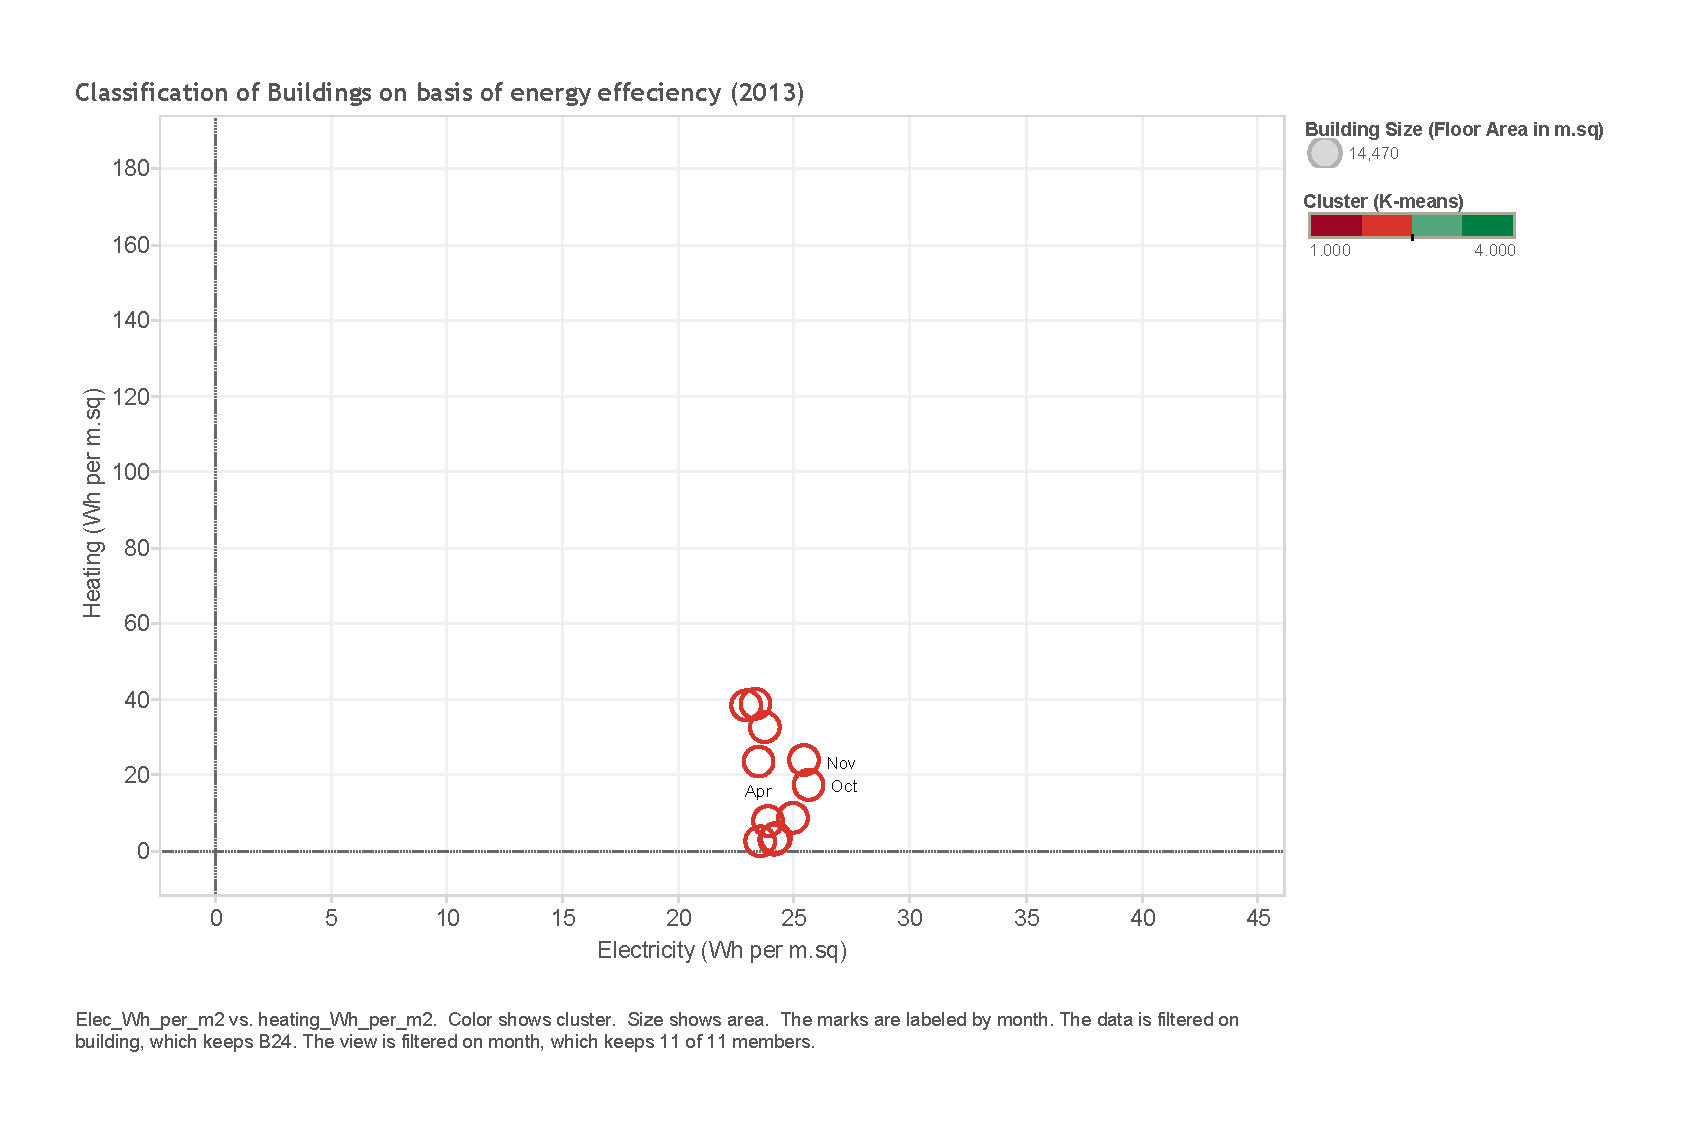
\includegraphics[width=\textwidth]{images/kmeans_b24_no.pdf}
                        \caption{Building 24: No Shift}
                        \label{fig:single}
       \end{subfigure}
     \caption{Energy effeciency cluster shift during 11 months}\label{fig:clustershift}
\end{figure}

An interactive dashboard is available for viewing the behaviour of all the buildings in the 11 months of collected data via following web address:

\url{http://catalyc.net/}

\section{Prediction models for forecasting energy consumption of household devices}
We discussed the data set collected by NIALM devices in section \ref{nialmset}. Using this data set we tried to evaluate different prediction models using limited amount of our data set. There were nine different appliances included in our data set i.e. Refrigerator, Freezer, Dishwasher, Laundry machine, Coffee maker, Stove, TV or PC, and Microwave oven. Some of the devices are generally in the continuous use e.g. freezer and refrigerator. While others are used on the need basis e.g. stove, coffee maker, laundry machine etc. Even in such devices, frequency of usage can be different e.g. stove, coffee maker etc. are usually used on daily basis while laundry machine can be used once in a week. The limited use of the data set means that we are not dealing with all this diversity. Instead we forecast only for those devices which are in continuous usage e.g. freezer and the refrigerator. The predicted values are on the daily consumption basis for a particular device.  
\subsection{Important considerations for forecasting}
Following were some of the important considerations while evaluating the prediction model.
\begin{enumerate}
\item We collected NIALM data in two phases. The first data set contained consumption values from 1st May 2013 to 3rd February 2014. This data was used as training data for prediction models. While the seconds data was collected with consumption values from 4th February 2014 till 30th April 2014. This set was used as the test data to measure the accuracy of the prediction model.
\item Predictions models were evaluated using consumption data of the freezer usage.
\item A time window of previous 30 days was used to predict the values for next 30 days with 80\% confidence interval.
\item  The accuracy of the prediction models were compared on basis of mean absolute error (MAE).
\end{enumerate}     

\subsection{Data processing steps}
Following are the main steps that were performed to evaluate the prediction models.

\begin{enumerate}
\item Data was reshaped to form continuous time series. The missing daily values were filled with zeros.
\item Data was aggregated to calculate the daily consumption for each device.
\item  The freezer data was extracted from the processed data set to apply the prediction models.
\item  Three forecasting models were applied to the training data i.e. Linear Regression, ARIMA, and Artificial Neural Networks (AAN). We used R for the ARIMA modeling and Weka for the Linear Regression and AAN. We shall discuss about the usage of these tools in chapter \ref{chapter:discussion}. 
\item We calculated the accuracy using test data and mean absolute error formula.  
\end{enumerate} 

\subsection{Forecasting results}

Figure \ref{fig:predicted} shows the resulting forecasts from the three prediction models. In figure~\ref{fig:arima}, predicted values using ARIMA model with 80\% confidence interval  are represented by the bold blue line, while shaded geom represent the higher and lower 80\% and 95\% confidence intervals respectively. The figures \ref{fig:lr} and \ref{fig:ann} illustrate the predictions using linear regression and artificial neural networks (ANN) models respectively using the 80\% confidence interval. Circular dots in the graphs show the predicted daily values, while the doted lines represent the higher and lower 80\% confidence interval prediction ranges. Due to the use of different analysis tools, the ARIMA graph is different from the linear regression and ANN graphs. Both the X axis and Y axis in all the graphs represents days and electricity  (Watt.hour) respectively. However label of the days in the X axis is in the figure \ref{fig:arima} is showing respective months with year while the label in the figures \ref{fig:lr} and \ref{fig:ann} represents the number of the day starting from the first day in the data.  
 \\
\begin{figure}
        \centering
        \begin{subfigure}[b]{\textwidth}
                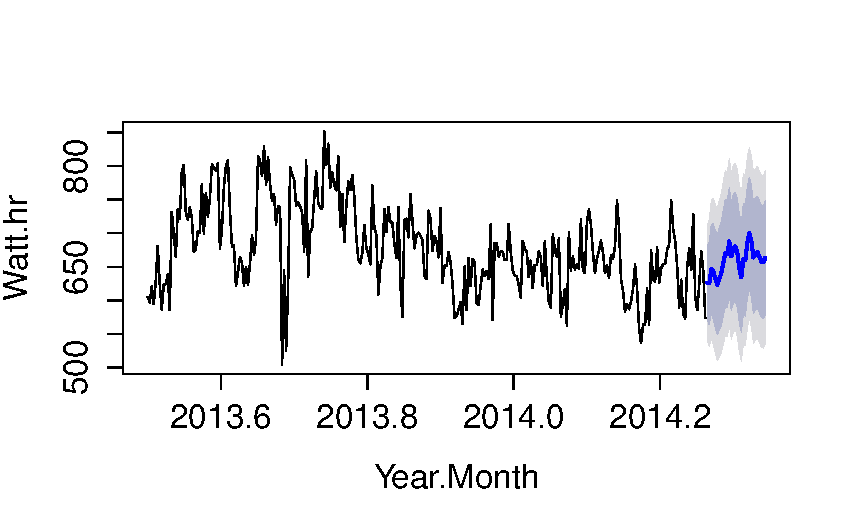
\includegraphics[width=\textwidth]{images/arima.pdf}
                \caption{ARIMA with 30 days AR and MA}
                \label{fig:arima}
        \end{subfigure}
        \\--------------------------------------------------
        
        
        \begin{subfigure}[b]{\textwidth}
                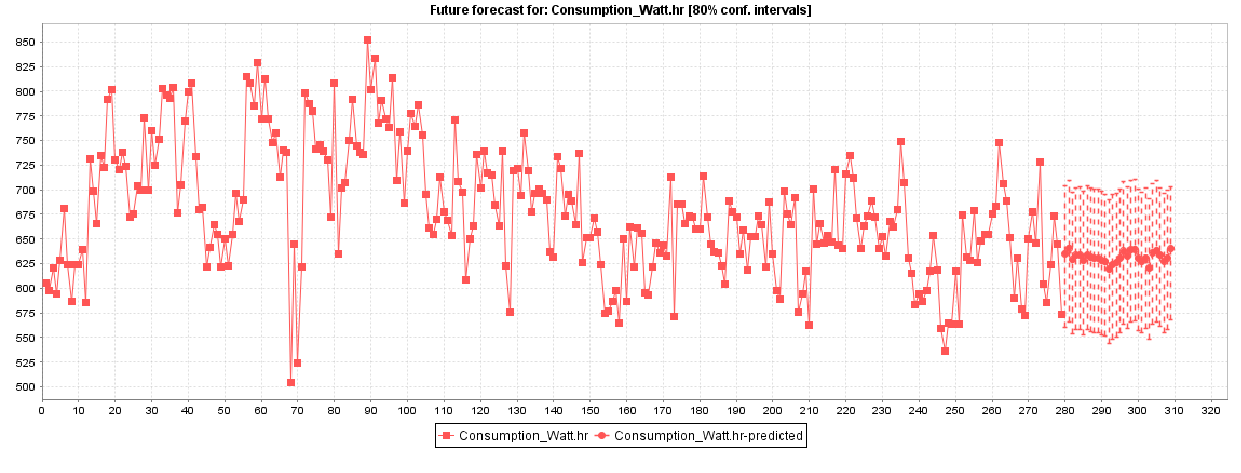
\includegraphics[width=\textwidth]{images/lr.pdf}
                \caption{Linear Regression Model}
                \label{fig:lr}
        \end{subfigure}
        \\---------------------------------------------------
        
        
        \begin{subfigure}[b]{\textwidth}
                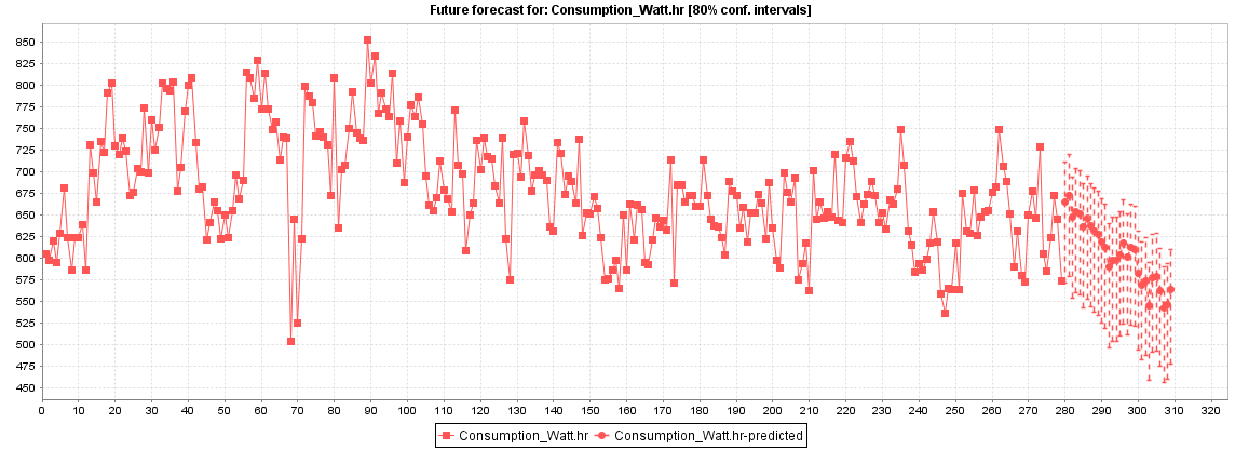
\includegraphics[width=\textwidth]{images/ann.pdf}
                \caption{Artificial Neural Network Model}
                \label{fig:ann}
        \end{subfigure}
             \caption{Forecasting monthly energy consumption for the home appliances based on previous monthly consumptions}\label{fig:predicted}
\end{figure}

Table \ref{tab:mae} lists the mean absolute error (MAE) values for each prediction model using 80\% confidence interval. Forecasting with the ARIMA model shows the lowest MAE values. For this reason, we included ARIMA forecasting as part of our implemented platform. We use R to perform calculations described in the section \ref{ARIMA} using packages like ``Forecast'' for fitting and forecasting with the ARIMA model and ``zoo'' for handling time series data structures. The p,d,q values for predicting monthly values based the previous 30 days were 30,0,30 respectively.

\begin{center}
\begin{table}[!ht] 
\begin{tabular} { | l | c | c | c | } 

\hline
	 & ARIMA & ANN & Linear Regression \\ \hline
	Mean Absolute Error (MAE) & 32.6 & 47.5 & 42.4 \\ \hline
\end{tabular}
\caption{Mean absolute error values for prediction models.}
\label{tab:mae}
\end{table}
\end{center}

  